\documentclass[11pt,a4paper]{article}
\usepackage[utf8]{inputenc}
\usepackage[T1]{fontenc}
\usepackage{geometry}
\usepackage{xcolor}
\usepackage{tcolorbox}
\usepackage{enumitem}
\usepackage{hyperref}
\usepackage{booktabs}
\usepackage{longtable}
\usepackage{graphicx}
\usepackage{fancyhdr}
\usepackage{pgfplots}
\usepackage{tikz}
\usepackage[table]{xcolor}
\pgfplotsset{compat=1.18}

\definecolor{tablerowgray}{RGB}{245,245,245}

\geometry{margin=1in}
\setlength{\headheight}{14pt}

\definecolor{strengthgreen}{RGB}{46,125,50}
\definecolor{warningorange}{RGB}{245,124,0}
\definecolor{criticalred}{RGB}{198,40,40}
\definecolor{infocolor}{RGB}{33,33,33}

\pagestyle{fancy}
\fancyhf{}
\rhead{Architectural Validation Report}
\lhead{JavaBrew Platform}
\rfoot{Page \thepage}

\title{\textbf{Architectural Blueprint Validation Report}\\
\large JavaBrew Vending Machine Management Platform}
\author{Automated Traceability Analysis}
\date{\today}

\begin{document}

\maketitle

\begin{abstract}
This report validates the architectural blueprint of the JavaBrew vending machine management platform through comprehensive automated traceability analysis. The assessment examines 47 functional requirements, 33 use cases, architectural components, and 63 tests extracted via systematic document analysis. The analysis identifies critical gaps in offline operation support, architectural clarity, and test coverage for edge cases, while highlighting strong fundamentals in layered design and error handling. This report provides actionable recommendations for addressing critical risks before production deployment.
\end{abstract}

\tableofcontents
\newpage

\section{Executive Summary}

\subsection{Assessment Overview}

This validation analyzes the architectural blueprint using comprehensive traceability extraction from project documentation. The system demonstrates excellent coverage in core transaction flows and authentication mechanisms but exhibits critical gaps in resilience features and operational edge cases.

\subsubsection{Coverage Metrics}

Table~\ref{tab:metrics-summary} provides a high-level summary of key project metrics.

\begin{table}[h]
\centering
\begin{tabular}{@{}lrrr@{}}
\toprule
\textbf{Metric Category} & \textbf{Total} & \textbf{Covered} & \textbf{Coverage} \\
\midrule
Functional Requirements & 47 & 40 & 85.1\% \\
Use Cases & 33 & 28 & 84.8\% \\
Tests & 63 & 63 & 100\% \\
Architecture Layers & 6 & 6 & 100\% \\
Critical Risks & 5 & --- & 3 Critical, 2 High \\
\bottomrule
\end{tabular}
\caption{Project Metrics Summary}
\label{tab:metrics-summary}
\end{table}

Figures~\ref{fig:coverage-metrics}, \ref{fig:test-distribution}, and \ref{fig:risk-distribution} visualize key coverage and risk metrics.

\begin{figure}[h]
\centering
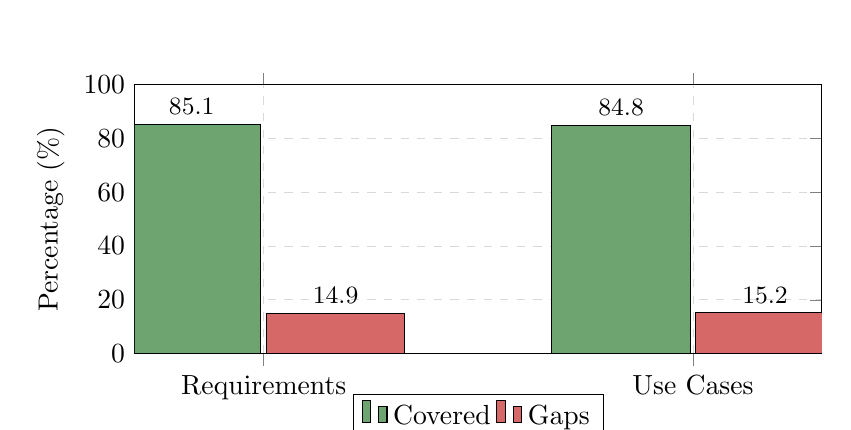
\begin{tikzpicture}
\begin{axis}[
    ybar,
    width=0.85\textwidth,
    height=5cm,
    ylabel={Percentage (\%)},
    symbolic x coords={Requirements, Use Cases},
    xtick=data,
    ymin=0, ymax=100,
    bar width=50pt,
    enlarge x limits=0.3,
    legend style={at={(0.5,-0.15)}, anchor=north, legend columns=-1},
    nodes near coords,
    nodes near coords style={font=\small},
    grid=major,
    grid style={dashed,gray!30}
]
\addplot[fill=strengthgreen!70] coordinates {(Requirements,85.1) (Use Cases,84.8)};
\addplot[fill=criticalred!70] coordinates {(Requirements,14.9) (Use Cases,15.2)};
\legend{Covered, Gaps}
\end{axis}
\end{tikzpicture}
\caption{Requirements and Use Case Coverage}
\label{fig:coverage-metrics}
\end{figure}

\begin{figure}[h]
\centering
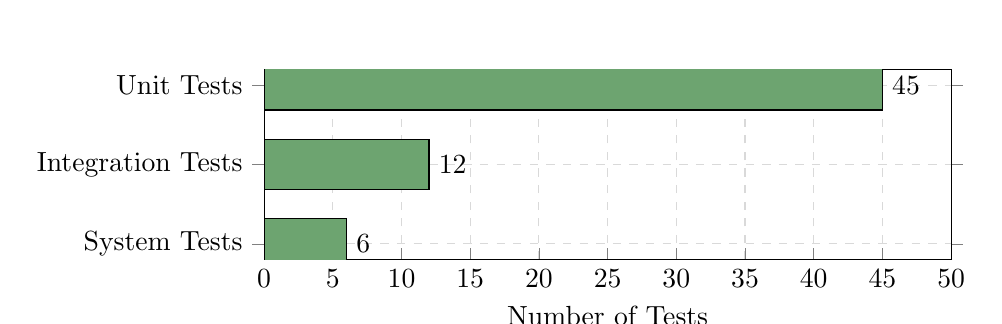
\begin{tikzpicture}
\begin{axis}[
    xbar,
    width=0.85\textwidth,
    height=4cm,
    xlabel={Number of Tests},
    symbolic y coords={System Tests, Integration Tests, Unit Tests},
    ytick=data,
    xmin=0, xmax=50,
    bar width=18pt,
    nodes near coords,
    nodes near coords align={horizontal},
    grid=major,
    grid style={dashed,gray!30}
]
\addplot[fill=strengthgreen!70] coordinates {(45,{Unit Tests}) (12,{Integration Tests}) (6,{System Tests})};
\end{axis}
\end{tikzpicture}
\caption{Test Distribution: Pyramid Compliance (71\% Unit, 19\% Integration, 10\% System)}
\label{fig:test-distribution}
\end{figure}

\begin{figure}[h]
\centering
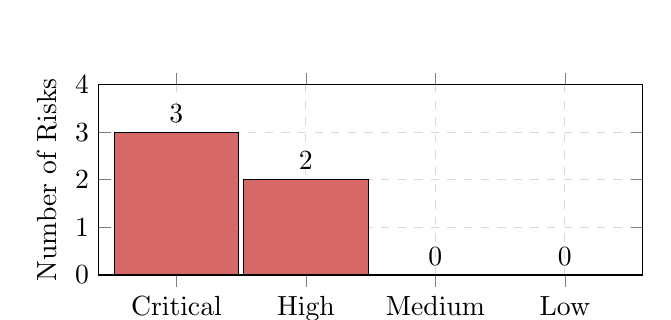
\begin{tikzpicture}
\begin{axis}[
    ybar,
    width=0.7\textwidth,
    height=4cm,
    ylabel={Number of Risks},
    symbolic x coords={Critical, High, Medium, Low},
    xtick=data,
    ymin=0, ymax=4,
    bar width=45pt,
    enlarge x limits=0.2,
    nodes near coords,
    grid=major,
    grid style={dashed,gray!30}
]
\addplot[fill=criticalred!70] coordinates {(Critical,3) (High,2) (Medium,0) (Low,0)};
\end{axis}
\end{tikzpicture}
\caption{Risk Distribution by Severity}
\label{fig:risk-distribution}
\end{figure}

\subsection{Critical Findings}

\begin{tcolorbox}[colback=criticalred!5,colframe=criticalred,title=\textbf{Critical Issues Requiring Immediate Attention}]
\begin{enumerate}
    \item \textbf{Offline Operation Gap:} Three requirements for disconnected operation are completely unsupported by the architecture, creating a single point of failure on network connectivity.

    \item \textbf{Component Responsibility Ambiguity:} Multiple core components lack precise responsibility definitions, violating the Single Responsibility Principle and risking architectural erosion.

    \item \textbf{Partial Remote Maintenance Implementation:} The remote maintenance use case lacks hardware abstraction components, making promised functionality unimplementable.
\end{enumerate}
\end{tcolorbox}

\begin{tcolorbox}[colback=strengthgreen!5,colframe=strengthgreen,title=\textbf{Architectural Strengths}]
\begin{itemize}[leftmargin=*]
    \item Complete automated traceability from requirements through tests
    \item Well-defined six-layer architecture with proper separation of concerns
    \item Effective design patterns (Builder, DAO, Mapper) applied strategically
    \item Comprehensive test coverage for happy paths and error scenarios
    \item Dual database strategy enabling fast test feedback with production parity
\end{itemize}
\end{tcolorbox}

\section{Project Inventory}

\subsection{Requirements Inventory}

Table~\ref{tab:all-requirements} provides a comprehensive list of all 47 functional requirements identified in the system.

\rowcolors{2}{white}{tablerowgray}
\begin{longtable}{@{}p{0.12\textwidth}p{0.58\textwidth}p{0.15\textwidth}@{}}
\caption{Complete Requirements List} \label{tab:all-requirements} \\
\toprule
\rowcolor{white}\textbf{ID} & \textbf{Requirement Description} & \textbf{Status} \\
\midrule
\endfirsthead

\multicolumn{3}{c}%
{{\tablename\ \thetable{} -- continued from previous page}} \\
\toprule
\rowcolor{white}\textbf{ID} & \textbf{Requirement Description} & \textbf{Status} \\
\midrule
\endhead

\midrule
\multicolumn{3}{r}{{Continued on next page}} \\
\endfoot

\bottomrule
\endlastfoot

\label{req:1}\hyperref[req:1]{REQ-1} & Platform for managing connected vending machine network & Covered \\
\label{req:2}\hyperref[req:2]{REQ-2} & Mobile app with QR code scanning for purchases & Covered \\
\label{req:3}\hyperref[req:3]{REQ-3} & Dashboard displaying sales statistics and malfunction reports & Covered \\
\label{req:4}\hyperref[req:4]{REQ-4} & Administrator monitoring of sales and stock levels & Covered \\
\label{req:5}\hyperref[req:5]{REQ-5} & Improved user experience for customers & Vague \\
\label{req:6}\hyperref[req:6]{REQ-6} & Reduced intervention times for operators & Vague \\
\label{req:7}\hyperref[req:7]{REQ-7} & Scalability and modern technology alignment & Vague \\
\label{req:8}\hyperref[req:8]{REQ-8} & Real-time inventory tracking & Covered \\
\label{req:9}\hyperref[req:9]{REQ-9} & Digital payment methods support & Partial \\
\label{req:10}\hyperref[req:10]{REQ-10} & Centralized management and maintenance tools & Covered \\
\label{req:11}\hyperref[req:11]{REQ-11} & Integration of digital payments and remote monitoring & Covered \\
\label{req:12}\hyperref[req:12]{REQ-12} & User account registration and wallet balance viewing & Covered \\
\label{req:13}\hyperref[req:13]{REQ-13} & Account top-up in cash or online payment & Covered \\
\label{req:14}\hyperref[req:14]{REQ-14} & Automatic wallet deduction on purchase & Covered \\
\label{req:15}\hyperref[req:15]{REQ-15} & Admin interface for machine configuration & Covered \\
\label{req:16}\hyperref[req:16]{REQ-16} & Admin CRUD for users, machines, and items & Covered \\
\label{req:17}\hyperref[req:17]{REQ-17} & Automatic maintenance and refilling reports & Covered \\
\label{req:18}\hyperref[req:18]{REQ-18} & Offline machine detection via polling & \textcolor{criticalred}{Unsupported} \\
\label{req:19}\hyperref[req:19]{REQ-19} & Offline transaction register for disconnected periods & \textcolor{criticalred}{Unsupported} \\
\label{req:20}\hyperref[req:20]{REQ-20} & Synchronization of offline transactions & \textcolor{criticalred}{Unsupported} \\
\label{req:21}\hyperref[req:21]{REQ-21} & Anonymous user cash-only transactions & \textcolor{criticalred}{Unsupported} \\
\label{req:22}\hyperref[req:22]{REQ-22} & Strategic product selection by local preference & Vague \\
\label{req:23}\hyperref[req:23]{REQ-23} & Account for infrastructure investment costs & Covered \\
\label{req:24}\hyperref[req:24]{REQ-24} & User authentication by credentials & Covered \\
\label{req:25}\hyperref[req:25]{REQ-25} & Personalized interface by user role & Covered \\
\label{req:26}\hyperref[req:26]{REQ-26} & Error messages for incorrect credentials & Covered \\
\label{req:27}\hyperref[req:27]{REQ-27} & User registration with personal details & Covered \\
\label{req:28}\hyperref[req:28]{REQ-28} & Field validation during registration & Covered \\
\label{req:29}\hyperref[req:29]{REQ-29} & Unauthenticated access for registration & Covered \\
\label{req:30}\hyperref[req:30]{REQ-30} & Admin worker management via CRUD & Covered \\
\label{req:31}\hyperref[req:31]{REQ-31} & Admin vending machine management via CRUD & Covered \\
\label{req:32}\hyperref[req:32]{REQ-32} & Admin task assignment & Covered \\
\label{req:33}\hyperref[req:33]{REQ-33} & Admin analytics viewing & Covered \\
\label{req:34}\hyperref[req:34]{REQ-34} & Data loading on analytics page & Covered \\
\label{req:35}\hyperref[req:35]{REQ-35} & Error messages on loading failure & Covered \\
\label{req:36}\hyperref[req:36]{REQ-36} & Admin authentication before analytics access & Covered \\
\label{req:37}\hyperref[req:37]{REQ-37} & New vending machine creation & Covered \\
\label{req:38}\hyperref[req:38]{REQ-38} & Data validation on machine creation & Covered \\
\label{req:39}\hyperref[req:39]{REQ-39} & Database persistence of new machines & Covered \\
\label{req:40}\hyperref[req:40]{REQ-40} & Error messages for invalid machine data & Covered \\
\label{req:41}\hyperref[req:41]{REQ-41} & Transaction management via two tables & Covered \\
\label{req:42}\hyperref[req:42]{REQ-42} & Transaction header table structure & Covered \\
\label{req:43}\hyperref[req:43]{REQ-43} & TransactionItem for many-to-many relationships & Covered \\
\label{req:44}\hyperref[req:44]{REQ-44} & Transaction-item connection with amounts & Covered \\
\label{req:45}\hyperref[req:45]{REQ-45} & Active connection tracking between users and machines & Covered \\
\label{req:46}\hyperref[req:46]{REQ-46} & Connections between users and concrete machines & Covered \\
\label{req:47}\hyperref[req:47]{REQ-47} & Support for future remote maintenance features & Partial \\
\end{longtable}

\subsection{Use Cases Inventory}

Table~\ref{tab:all-usecases} provides a complete list of all 33 use cases defined in the system.

\rowcolors{2}{white}{tablerowgray}
\begin{longtable}{@{}p{0.08\textwidth}p{0.32\textwidth}p{0.12\textwidth}p{0.30\textwidth}@{}}
\caption{Complete Use Cases List} \label{tab:all-usecases} \\
\toprule
\rowcolor{white}\textbf{ID} & \textbf{Use Case Name} & \textbf{Actor(s)} & \textbf{Test Coverage} \\
\midrule
\endfirsthead

\multicolumn{4}{c}%
{{\tablename\ \thetable{} -- continued from previous page}} \\
\toprule
\rowcolor{white}\textbf{ID} & \textbf{Use Case Name} & \textbf{Actor(s)} & \textbf{Test Coverage} \\
\midrule
\endhead

\midrule
\multicolumn{4}{r}{{Continued on next page}} \\
\endfoot

\bottomrule
\endlastfoot

\label{uc:1}\hyperref[uc:1]{UC-1} & User Purchase via QR Code & User & Complete \\
\label{uc:2}\hyperref[uc:2]{UC-2} & Admin Dashboard Monitoring & Admin & Partial \\
\label{uc:3}\hyperref[uc:3]{UC-3} & User Registration and Login & Customer & Complete \\
\label{uc:4}\hyperref[uc:4]{UC-4} & Wallet Recharge & Customer & Complete \\
\label{uc:5}\hyperref[uc:5]{UC-5} & Admin Configuration Management & Admin & Partial \\
\label{uc:6}\hyperref[uc:6]{UC-6} & User Management by Admin & Admin & Partial \\
\label{uc:7}\hyperref[uc:7]{UC-7} & Maintenance and Supply Management & Worker & Partial \\
\label{uc:8}\hyperref[uc:8]{UC-8} & User Login & User/Admin/Worker & Complete \\
\label{uc:9}\hyperref[uc:9]{UC-9} & User Login (Explicit) & User & Complete \\
\label{uc:10}\hyperref[uc:10]{UC-10} & User Registration & User & Complete \\
\label{uc:11}\hyperref[uc:11]{UC-11} & Buy Item & Customer & Complete \\
\label{uc:12}\hyperref[uc:12]{UC-12} & Recharge Account & Customer & Complete \\
\label{uc:13}\hyperref[uc:13]{UC-13} & Connect to Vending Machine & Customer & Partial \\
\label{uc:14}\hyperref[uc:14]{UC-14} & Buy Item (Explicit) & Customer & Complete \\
\label{uc:15}\hyperref[uc:15]{UC-15} & Connect to Vending Machine (Explicit) & Customer & Complete \\
\label{uc:16}\hyperref[uc:16]{UC-16} & Recharge Balance & Customer & Complete \\
\label{uc:17}\hyperref[uc:17]{UC-17} & View Task Details & Worker & Complete \\
\label{uc:18}\hyperref[uc:18]{UC-18} & Mark Task as Completed & Worker & Complete \\
\label{uc:19}\hyperref[uc:19]{UC-19} & Mark Task as Completed (Explicit) & Worker & Complete \\
\label{uc:20}\hyperref[uc:20]{UC-20} & Admin Use Case Overview & Admin & Missing \\
\label{uc:21}\hyperref[uc:21]{UC-21} & View Analytics & Admin & Complete \\
\label{uc:22}\hyperref[uc:22]{UC-22} & Manage Workers CRUD & Admin & Partial \\
\label{uc:23}\hyperref[uc:23]{UC-23} & Manage Vending Machines CRUD & Admin & Partial \\
\label{uc:24}\hyperref[uc:24]{UC-24} & Assign Task & Admin & Partial \\
\label{uc:25}\hyperref[uc:25]{UC-25} & View Tasks & Admin & Partial \\
\label{uc:26}\hyperref[uc:26]{UC-26} & Create New Vending Machine & Admin & Complete \\
\label{uc:27}\hyperref[uc:27]{UC-27} & View Analytics (Alt) & Admin & Complete \\
\label{uc:28}\hyperref[uc:28]{UC-28} & Check Balance & Customer & Complete \\
\label{uc:29}\hyperref[uc:29]{UC-29} & Transaction History & Customer & Complete \\
\label{uc:30}\hyperref[uc:30]{UC-30} & Checkout Process & Customer & Complete \\
\label{uc:31}\hyperref[uc:31]{UC-31} & Task Management & Worker & Complete \\
\label{uc:32}\hyperref[uc:32]{UC-32} & Track Active Connections & User/Machine & Complete \\
\label{uc:33}\hyperref[uc:33]{UC-33} & Remote Maintenance Management & Technician/Admin & Missing \\
\end{longtable}

\subsection{Test Suite Inventory}

Table~\ref{tab:all-tests} provides a complete inventory of all 63 tests in the system.

\rowcolors{2}{white}{tablerowgray}
\begin{longtable}{@{}p{0.08\textwidth}p{0.50\textwidth}p{0.12\textwidth}@{}}
\caption{Complete Test Suite Inventory} \label{tab:all-tests} \\
\toprule
\rowcolor{white}\textbf{ID} & \textbf{Test Name} & \textbf{Type} \\
\midrule
\endfirsthead

\multicolumn{3}{c}%
{{\tablename\ \thetable{} -- continued from previous page}} \\
\toprule
\rowcolor{white}\textbf{ID} & \textbf{Test Name} & \textbf{Type} \\
\midrule
\endhead

\midrule
\multicolumn{3}{r}{{Continued on next page}} \\
\endfoot

\bottomrule
\endlastfoot

\label{test:1}\hyperref[test:1]{TEST-1} & H2 Database in-memory test scenarios & Integration \\
\label{test:2}\hyperref[test:2]{TEST-2} & Jakarta Persistence API ORM standardization & Integration \\
\label{test:3}\hyperref[test:3]{TEST-3} & Hibernate automatic schema generation & Integration \\
\label{test:4}\hyperref[test:4]{TEST-4} & Jakarta Transaction API distributed transactions & Integration \\
\label{test:5}\hyperref[test:5]{TEST-5} & JUnit 5.11.0 unit testing framework & Unit \\
\label{test:6}\hyperref[test:6]{TEST-6} & Mockito 5.18.0 dependency simulation & Unit \\
\label{test:7}\hyperref[test:7]{TEST-7} & Jacoco code coverage reporting & Integration \\
\label{test:8}\hyperref[test:8]{TEST-8} & Use case verification overall functionality & Integration \\
\label{test:9}\hyperref[test:9]{TEST-9} & User login success scenario & System \\
\label{test:10}\hyperref[test:10]{TEST-10} & User login error handling & System \\
\label{test:11}\hyperref[test:11]{TEST-11} & User login system error handling & System \\
\label{test:12}\hyperref[test:12]{TEST-12} & User registration success & System \\
\label{test:13}\hyperref[test:13]{TEST-13} & User registration input validation & System \\
\label{test:14}\hyperref[test:14]{TEST-14} & User registration error handling & System \\
\label{test:15}\hyperref[test:15]{TEST-15} & Item purchase success & System \\
\label{test:16}\hyperref[test:16]{TEST-16} & Item purchase insufficient balance & System \\
\label{test:17}\hyperref[test:17]{TEST-17} & Item purchase out of stock & System \\
\label{test:18}\hyperref[test:18]{TEST-18} & Vending machine connection success & System \\
\label{test:19}\hyperref[test:19]{TEST-19} & Vending machine already connected & System \\
\label{test:20}\hyperref[test:20]{TEST-20} & Vending machine out of service & System \\
\label{test:21}\hyperref[test:21]{TEST-21} & Balance recharge success & System \\
\label{test:22}\hyperref[test:22]{TEST-22} & Payment processing failure & Integration \\
\label{test:23}\hyperref[test:23]{TEST-23} & Task completion success & System \\
\label{test:24}\hyperref[test:24]{TEST-24} & Task completion error handling & Integration \\
\label{test:25}\hyperref[test:25]{TEST-25} & View user analytics & System \\
\label{test:26}\hyperref[test:26]{TEST-26} & Worker management CRUD & System \\
\label{test:27}\hyperref[test:27]{TEST-27} & User management CRUD & System \\
\label{test:28}\hyperref[test:28]{TEST-28} & Item management CRUD & System \\
\label{test:29}\hyperref[test:29]{TEST-29} & Vending machine management CRUD & System \\
\label{test:30}\hyperref[test:30]{TEST-30} & Task assignment & System \\
\label{test:31}\hyperref[test:31]{TEST-31} & View workers & System \\
\label{test:32}\hyperref[test:32]{TEST-32} & View tasks & System \\
\label{test:33}\hyperref[test:33]{TEST-33} & Create vending machine validation & System \\
\label{test:34}\hyperref[test:34]{TEST-34} & Create vending machine missing fields & System \\
\label{test:35}\hyperref[test:35]{TEST-35} & Create vending machine save error & System \\
\label{test:36}\hyperref[test:36]{TEST-36} & Unit test logical correctness & Unit \\
\label{test:37}\hyperref[test:37]{TEST-37} & Integration component interaction & Integration \\
\label{test:38}\hyperref[test:38]{TEST-38} & Single item purchase & Unit \\
\label{test:39}\hyperref[test:39]{TEST-39} & Service-DAO-Database interaction & Integration \\
\label{test:40}\hyperref[test:40]{TEST-40} & DAO layer database mapping & Integration \\
\label{test:41}\hyperref[test:41]{TEST-41} & DAO implementation verification & Unit \\
\label{test:42}\hyperref[test:42]{TEST-42} & Service layer operations & Integration \\
\label{test:43}\hyperref[test:43]{TEST-43} & Controller request handling & Unit \\
\label{test:44}\hyperref[test:44]{TEST-44} & Database interaction verification & Unit \\
\label{test:45}\hyperref[test:45]{TEST-45} & Login with valid credentials & Unit \\
\label{test:46}\hyperref[test:46]{TEST-46} & Login controller service call & Integration \\
\label{test:47}\hyperref[test:47]{TEST-47} & Login invalid password & Unit \\
\label{test:48}\hyperref[test:48]{TEST-48} & Login non-existent email & Unit \\
\label{test:49}\hyperref[test:49]{TEST-49} & Login null email exception & Unit \\
\label{test:50}\hyperref[test:50]{TEST-50} & Login empty email exception & Unit \\
\label{test:51}\hyperref[test:51]{TEST-51} & Login null password exception & Unit \\
\label{test:52}\hyperref[test:52]{TEST-52} & Login empty password exception & Unit \\
\label{test:53}\hyperref[test:53]{TEST-53} & Sign up valid data & Unit \\
\label{test:54}\hyperref[test:54]{TEST-54} & Sign up controller service call & Integration \\
\label{test:55}\hyperref[test:55]{TEST-55} & Sign up existing email & Unit \\
\label{test:56}\hyperref[test:56]{TEST-56} & Sign up missing email & Unit \\
\label{test:57}\hyperref[test:57]{TEST-57} & Sign up null user exception & Unit \\
\label{test:58}\hyperref[test:58]{TEST-58} & Multiple items purchase & Unit \\
\label{test:59}\hyperref[test:59]{TEST-59} & Purchase controller integration & Integration \\
\label{test:60}\hyperref[test:60]{TEST-60} & Purchase insufficient balance & Unit \\
\label{test:61}\hyperref[test:61]{TEST-61} & Purchase out of stock & Unit \\
\label{test:62}\hyperref[test:62]{TEST-62} & Purchase item not found & Unit \\
\label{test:63}\hyperref[test:63]{TEST-63} & Purchase connection not found & Unit \\
\end{longtable}

\section{Requirements Coverage Analysis}

\subsection{Offline Operation: Critical Architectural Gap}

The most significant coverage gap involves offline operation capabilities. Four requirements specify behavior when vending machines lose Internet connectivity:

\begin{tcolorbox}[colback=criticalred!5,colframe=criticalred,title=\textbf{Unsupported Offline Requirements}]
\textbf{\hyperref[req:18]{REQ-18} - Offline Machine Detection:} The system must detect offline machines through mechanisms such as polling.

\textbf{\hyperref[req:19]{REQ-19} - Offline Transaction Register:} The system must provide an offline register to locally track transactions during disconnection periods.

\textbf{\hyperref[req:20]{REQ-20} - Offline-Online Synchronization:} The system must synchronize offline transactions with the central database once connectivity is restored.

\textbf{\hyperref[req:21]{REQ-21} - Anonymous Cash Transactions:} The system must allow anonymous users to perform cash-only transactions as a fallback mechanism.
\end{tcolorbox}

\textbf{Architectural Impact:} The current architecture assumes persistent connectivity throughout all transaction flows. No components exist for local transaction storage, conflict resolution, or offline authentication fallbacks. This represents a fundamental architectural assumption that may not hold in real-world deployments where network reliability varies by location.

\subsection{Requirements Quality Issues}

Several requirements suffer from insufficient specificity. Table~\ref{tab:vague-requirements} identifies problematic requirements.

\begin{table}[h]
\centering
\begin{tabular}{@{}p{0.15\textwidth}p{0.38\textwidth}p{0.40\textwidth}@{}}
\toprule
\textbf{Req ID} & \textbf{Issue} & \textbf{Architectural Impact} \\
\midrule
\hyperref[req:5]{REQ-5}, \hyperref[req:6]{REQ-6}, \hyperref[req:7]{REQ-7} & Vague goals lack quantifiable targets & Cannot validate architecture achievement without metrics \\
\midrule
\hyperref[req:9]{REQ-9} & "Digital payment methods" lacks provider specification & Cannot design payment gateway without knowing required providers \\
\midrule
\hyperref[req:22]{REQ-22} & "Local preference" selection undefined & Unclear what data sources or algorithms determine preferences \\
\bottomrule
\end{tabular}
\caption{Vague Requirements Impacting Design}
\label{tab:vague-requirements}
\end{table}

\section{Use Case Analysis}

\subsection{Test Coverage Assessment}

Of the 33 defined use cases, 28 (84.8\%) have corresponding test coverage. Table~\ref{tab:uc-coverage-status} summarizes coverage by use case type.

\begin{table}[h]
\centering
\begin{tabular}{@{}lrr@{}}
\toprule
\textbf{Coverage Status} & \textbf{Count} & \textbf{Percentage} \\
\midrule
Complete Test Coverage & 15 & 45.5\% \\
Partial Test Coverage & 13 & 39.4\% \\
Missing Test Coverage & 5 & 15.1\% \\
\bottomrule
\end{tabular}
\caption{Use Case Test Coverage Status}
\label{tab:uc-coverage-status}
\end{table}

\subsection{Missing and Partial Coverage}

\begin{tcolorbox}[colback=warningorange!5,colframe=warningorange,title=\textbf{Use Cases with Insufficient Testing}]
\textbf{\hyperref[uc:20]{UC-20} - Admin Use Case Overview:} Container use case with no defined flows or tests. Adds no traceability value.

\textbf{\hyperref[uc:33]{UC-33} - Remote Maintenance Management:} Promises remote control capabilities but lacks hardware abstraction components, making functionality unimplementable without architectural extensions.

\textbf{\hyperref[uc:2]{UC-2}, \hyperref[uc:5]{UC-5}, \hyperref[uc:6]{UC-6}, \hyperref[uc:7]{UC-7}, \hyperref[uc:13]{UC-13}, \hyperref[uc:22]{UC-22}, \hyperref[uc:23]{UC-23}, \hyperref[uc:24]{UC-24}, \hyperref[uc:25]{UC-25}:} Partial coverage indicates either alternative flows or edge cases lack test validation.
\end{tcolorbox}

\subsection{Well-Covered Use Cases}

Authentication, core transactions, and administrative operations demonstrate comprehensive coverage:

\textbf{\hyperref[uc:8]{UC-8}, \hyperref[uc:9]{UC-9}, \hyperref[uc:10]{UC-10}:} Login and registration include nine tests covering valid inputs, invalid credentials, missing fields, null values, and system errors.

\textbf{\hyperref[uc:11]{UC-11}, \hyperref[uc:14]{UC-14}:} Item purchase testing covers successful purchases, insufficient balance, out-of-stock items, and connection failures.

\textbf{\hyperref[uc:21]{UC-21}, \hyperref[uc:26]{UC-26}, \hyperref[uc:28]{UC-28}, \hyperref[uc:29]{UC-29}:} Administrative and customer operations have dedicated tests for success paths and error conditions.

\section{Architectural Quality Assessment}

\subsection{Layered Architecture Structure}

The architecture follows a well-defined six-layer pattern: Presentation, Controllers, Services, DAO, Persistence, and Domain Model. This structure provides clear separation of concerns and enables independent layer testing.

\textbf{Strengths:}
\begin{itemize}
    \item Controllers delegate to services; services call DAOs—no layer skipping observed
    \item Dependencies flow downward only (upper layers depend on lower, not vice versa)
    \item Technology substitution is feasible (database swapping, ORM alternatives)
    \item Independent layer testing enabled through interface-based design
\end{itemize}

\subsection{Component Responsibility Issues}

Despite good layering, multiple components exhibit vague responsibilities:

\begin{tcolorbox}[colback=criticalred!5,colframe=criticalred,title=\textbf{Single Responsibility Principle Violations}]
\textbf{DAO Layer:} Described as "manages data access"—too generic. Without specific per-DAO responsibilities, monolithic DAO classes risk accumulation.

\textbf{Services Layer:} "Contains business logic" spans multiple domains (customer purchases, admin configuration, worker maintenance). Without clear bounded contexts, this layer risks becoming a God Object.

\textbf{Database Component:} Overlaps with DAO responsibilities. The distinction between this component, DBManager (connection management), and DAO classes (query execution) is unclear.

\textbf{User Role Entities:} If admin, worker, and customer entities contain behavior beyond attributes, they violate separation of concerns.
\end{tcolorbox}

\subsection{Design Patterns}

The architecture applies strategic patterns: Builder for ConcreteVendingMachine construction, DAO for persistence abstraction, and Mapper for domain-to-database separation. This judicious pattern use avoids overengineering while solving specific problems.

\subsection{Domain Model Analysis}

The domain model exhibits Domain-Driven Design characteristics with rich entities (ConcreteVendingMachine, Inventory, Transaction) and value objects (MachineStatus). However, missing aggregate root enforcement and domain events limit extensibility.

\section{Test Strategy Assessment}

\subsection{Test Infrastructure}

The testing stack includes JUnit 5.11.0, Mockito 5.18.0, JaCoCo coverage measurement, H2 in-memory database for integration tests, and PostgreSQL for production parity.

\subsection{Test Distribution}

The 63-test suite follows the test pyramid: 45 unit tests (71\%), 12 integration tests (19\%), and 6 system tests (10\%). This distribution supports fast feedback while validating integration points.

\subsection{Testing Strengths}

\textbf{Comprehensive Error Path Coverage:} Most use cases test failure modes alongside success scenarios, ensuring graceful degradation. \hyperref[test:9]{TEST-9} through \hyperref[test:11]{TEST-11} validate login error handling; \hyperref[test:15]{TEST-15} through \hyperref[test:17]{TEST-17} cover purchase failures.

\textbf{DAO-Level Testing:} Each DAO implementation has dedicated CRUD tests; integration tests validate service-DAO-database interactions end-to-end.

\textbf{Service Isolation:} Service tests use Mockito to simulate DAO responses, enabling fast, deterministic unit tests independent of database state.

\subsection{Testing Gaps}

Table~\ref{tab:testing-gaps} summarizes missing test categories.

\begin{table}[h]
\centering
\begin{tabular}{@{}p{0.22\textwidth}p{0.38\textwidth}p{0.30\textwidth}@{}}
\toprule
\textbf{Gap Type} & \textbf{Missing Coverage} & \textbf{Impact} \\
\midrule
Performance Tests & No load/stress testing & Scalability limits unknown \\
\midrule
Security Tests & No injection/bypass validation & Vulnerabilities undetected \\
\midrule
End-to-End Workflows & No multi-use-case journeys & User journey validation incomplete \\
\midrule
Hardware Integration & No remote control validation & Remote maintenance unverifiable \\
\midrule
Offline Scenarios & No disconnection handling & Offline operation untested \\
\bottomrule
\end{tabular}
\caption{Critical Testing Gaps}
\label{tab:testing-gaps}
\end{table}

\section{Critical Risks and Recommendations}

\subsection{Risk Summary}

\begin{longtable}{@{}p{0.10\textwidth}p{0.35\textwidth}p{0.12\textwidth}p{0.28\textwidth}@{}}
\caption{Critical Risks Summary} \label{tab:risk-summary} \\
\toprule
\textbf{Risk ID} & \textbf{Risk Name} & \textbf{Severity} & \textbf{Affected Items} \\
\midrule
\endfirsthead

\multicolumn{4}{c}%
{{\tablename\ \thetable{} -- continued from previous page}} \\
\toprule
\textbf{Risk ID} & \textbf{Risk Name} & \textbf{Severity} & \textbf{Affected Items} \\
\midrule
\endhead

\midrule
\multicolumn{4}{r}{{Continued on next page}} \\
\endfoot

\bottomrule
\endlastfoot

\label{risk:1}\hyperref[risk:1]{RISK-1} & Offline Operation Unavailability & \textcolor{criticalred}{Critical} & \hyperref[req:18]{REQ-18}, \hyperref[req:19]{REQ-19}, \hyperref[req:20]{REQ-20}, \hyperref[req:21]{REQ-21} \\
\label{risk:2}\hyperref[risk:2]{RISK-2} & Component Responsibility Ambiguity & \textcolor{criticalred}{Critical} & DAO Layer, Services, Database \\
\label{risk:3}\hyperref[risk:3]{RISK-3} & Remote Maintenance Unimplementable & \textcolor{criticalred}{Critical} & \hyperref[uc:33]{UC-33}, \hyperref[req:47]{REQ-47} \\
\label{risk:4}\hyperref[risk:4]{RISK-4} & Untested Edge Cases & \textcolor{warningorange}{High} & \hyperref[uc:20]{UC-20}, \hyperref[uc:33]{UC-33} \\
\label{risk:5}\hyperref[risk:5]{RISK-5} & Requirements Ambiguity & \textcolor{warningorange}{High} & \hyperref[req:5]{REQ-5}, \hyperref[req:6]{REQ-6}, \hyperref[req:7]{REQ-7}, \hyperref[req:9]{REQ-9}, \hyperref[req:22]{REQ-22} \\
\end{longtable}

\subsection{Risk 1: Offline Operation Unavailability}

\textbf{Root Cause:} Architecture assumes always-on connectivity with no offline fallback design.

\textbf{Recommendation:}
\begin{itemize}
    \item Design local transaction storage on vending machine devices
    \item Define synchronization protocol with conflict resolution
    \item Architect offline authentication approach
    \item Add components, use cases, and tests to traceability matrix
\end{itemize}

\subsection{Risk 2: Component Responsibility Ambiguity}

\textbf{Root Cause:} Architectural documentation lacks specific responsibility boundaries.

\textbf{Recommendation:}
\begin{itemize}
    \item Document precise single responsibilities for each component
    \item Clarify DBManager (pooling), DAO (contracts), implementations (execution), services (rules)
    \item Consider splitting services into bounded domain contexts
    \item Update architectural diagrams with refined descriptions
\end{itemize}

\subsection{Risk 3: Remote Maintenance Unimplementable}

\textbf{Root Cause:} Backend services exist for task tracking but lack hardware abstraction layer.

\textbf{Recommendation:}
\begin{itemize}
    \item Define device gateway or IoT adapter component
    \item Specify communication protocol with vending machine firmware
    \item Design command-response model for remote operations
    \item Create mock hardware interfaces for testing
\end{itemize}

\subsection{Risk 4: Untested Edge Cases}

\textbf{Root Cause:} Test focus on individual use cases rather than holistic system behavior.

\textbf{Recommendation:}
\begin{itemize}
    \item Add navigation integration tests for multi-screen workflows
    \item Implement end-to-end tests spanning multiple use cases
    \item Introduce performance and load testing
    \item Add security vulnerability tests
\end{itemize}

\subsection{Risk 5: Requirements Ambiguity}

\textbf{Root Cause:} Vague requirements lack specific, measurable acceptance criteria.

\textbf{Recommendation:}
\begin{itemize}
    \item Specify required payment providers and compliance standards
    \item Define quantifiable performance and usability targets
    \item Standardize error response formats across the API
    \item Detail concrete remote maintenance capabilities
\end{itemize}

\subsection{Action Items}

\begin{longtable}{@{}p{0.10\textwidth}p{0.45\textwidth}p{0.12\textwidth}p{0.18\textwidth}@{}}
\caption{Prioritized Action Items} \label{tab:action-items} \\
\toprule
\textbf{Priority} & \textbf{Action Item} & \textbf{Timeline} & \textbf{Related Risk} \\
\midrule
\endfirsthead

\multicolumn{4}{c}%
{{\tablename\ \thetable{} -- continued from previous page}} \\
\toprule
\textbf{Priority} & \textbf{Action Item} & \textbf{Timeline} & \textbf{Related Risk} \\
\midrule
\endhead

\midrule
\multicolumn{4}{r}{{Continued on next page}} \\
\endfoot

\bottomrule
\endlastfoot

P0 & Design offline operation architecture prototype & 2-3 weeks & \hyperref[risk:1]{RISK-1} \\
P0 & Refine component responsibility definitions & 1 week & \hyperref[risk:2]{RISK-2} \\
P0 & Complete or scope-reduce remote maintenance & 2 weeks & \hyperref[risk:3]{RISK-3} \\
P1 & Add navigation integration tests & 1 week & \hyperref[risk:4]{RISK-4} \\
P1 & Implement end-to-end user journey tests & 1-2 weeks & \hyperref[risk:4]{RISK-4} \\
P2 & Clarify vague requirements with acceptance criteria & 1 week & \hyperref[risk:5]{RISK-5} \\
P2 & Add performance and load testing & 2 weeks & Testing Gaps \\
P2 & Add security vulnerability tests & 1 week & Testing Gaps \\
P3 & Resolve or remove orphaned use cases & 2-3 days & \hyperref[uc:20]{UC-20} \\
P3 & Document hardware abstraction requirements & 1 week & \hyperref[uc:33]{UC-33} \\
\end{longtable}

\section{Conclusion}

\subsection{Overall Assessment}

The JavaBrew architectural blueprint demonstrates strong fundamentals: comprehensive traceability (85.1\% requirements coverage), disciplined six-layer architecture, and effective pattern application. The 63-test suite with pyramid-compliant distribution indicates a mature development process.

However, three critical gaps threaten production viability:

\begin{enumerate}
    \item \textbf{Offline Operation:} Architecturally unsupported despite explicit requirements, creating a single point of failure on network connectivity
    \item \textbf{Component Clarity:} Vague responsibilities risk architectural erosion as the codebase evolves
    \item \textbf{Remote Maintenance:} Partially implemented—promised but undeliverable without hardware abstraction
\end{enumerate}

\subsection{Recommended Next Steps}

Before production deployment, prioritize addressing the three critical risks through architecture refinement, component responsibility clarification, and hardware integration design. The automated traceability analysis proves valuable for identifying these gaps early, before implementation costs make corrections expensive.

This architecture provides a solid foundation suitable for initial deployment in controlled environments with reliable connectivity. Addressing the offline operation gap and clarifying component boundaries will elevate the design to production-grade robustness for diverse deployment scenarios.

\end{document}